%%%%%%%%%%%%%%%%%%%%%%%%%%%%%%%%%%%%%%%%%
% Short Sectioned Assignment
% LaTeX Template
% Version 1.0 (5/5/12)
%
% This template has been downloaded from:
% http://www.LaTeXTemplates.com
%
% Original author:
% Frits Wenneker (http://www.howtotex.com)
%
% License:
% CC BY-NC-SA 3.0 (http://creativecommons.org/licenses/by-nc-sa/3.0/)
%
%%%%%%%%%%%%%%%%%%%%%%%%%%%%%%%%%%%%%%%%%

%----------------------------------------------------------------------------------------
%	PACKAGES AND OTHER DOCUMENT CONFIGURATIONS
%----------------------------------------------------------------------------------------

\documentclass[paper=a4, fontsize=11pt]{scrartcl} % A4 paper and 11pt font size

\usepackage[T1]{fontenc} % Use 8-bit encoding that has 256 glyphs
\usepackage{fourier} % Use the Adobe Utopia font for the document - comment this line to return to the LaTeX default
\usepackage[english]{babel} % English language/hyphenation
\usepackage{amsmath,amsfonts,amsthm} % Math packages
\usepackage{listings}
\usepackage{graphicx}
\usepackage{float}
\usepackage{lipsum}
%\usepackage{minipage}
%\usepackage{subfig}
\usepackage{cite}
\usepackage{subcaption}
%\usepackage{epstopdf}
%\graphicspath{ {Desktop/PA3_numerical_analysis/} }

\usepackage{lipsum} % Used for inserting dummy 'Lorem ipsum' text into the template

\usepackage{sectsty} % Allows customizing section commands
\allsectionsfont{\centering \normalfont\scshape} % Make all sections centered, the default font and small caps

\usepackage{fancyhdr} % Custom headers and footers
\pagestyle{fancyplain} % Makes all pages in the document conform to the custom headers and footers
\fancyhead{} % No page header - if you want one, create it in the same way as the footers below
\fancyfoot[L]{} % Empty left footer
\fancyfoot[C]{} % Empty center footer
\fancyfoot[R]{\thepage} % Page numbering for right footer
\renewcommand{\headrulewidth}{0pt} % Remove header underlines
\renewcommand{\footrulewidth}{0pt} % Remove footer underlines
\setlength{\headheight}{13.6pt} % Customize the height of the header

\numberwithin{equation}{section} % Number equations within sections (i.e. 1.1, 1.2, 2.1, 2.2 instead of 1, 2, 3, 4)
\numberwithin{figure}{section} % Number figures within sections (i.e. 1.1, 1.2, 2.1, 2.2 instead of 1, 2, 3, 4)
\numberwithin{table}{section} % Number tables within sections (i.e. 1.1, 1.2, 2.1, 2.2 instead of 1, 2, 3, 4)

\setlength\parindent{0pt} % Removes all indentation from paragraphs - comment this line for an assignment with lots of text

%----------------------------------------------------------------------------------------
%	TITLE SECTION
%----------------------------------------------------------------------------------------

\newcommand{\horrule}[1]{\rule{\linewidth}{#1}} % Create horizontal rule command with 1 argument of height

\title{	
\normalfont \normalsize 
\textsc{The College of William and Mary} \\ [25pt] % Your university, school and/or department name(s)
\horrule{0.5pt} \\[0.4cm] % Thin top horizontal rule
\huge Newton's Method Applied to Systems of Nonlinear Equations \\ % The assignment title
\horrule{2pt} \\[0.5cm] % Thick bottom horizontal rule
}

\author{Alexander Powell} % Your name

\date{\normalsize May 12, 2015} % Today's date or a custom date

\begin{document}
\lstset{language=MATLAB}
\maketitle % Print the title

\theoremstyle{definition}
\newtheorem{exmp}{Example}[section]

\theoremstyle{definition}
\newtheorem{definition}{Definition}[section]


% -------BEGIN DOCUMENT----------%

\section{Abstract}
Newton's method is an iterative algorithm used to find the roots of nonlinear equations.  The method can also be further extended to entire systems of nonlinear equations.  Newton's root finding method has many benefits.  For one, it can be extremely fast when the input is a relatively good guess.  Also, some problems can be very difficult to solve for exactly, so the iterative technique exemplified in the newton method can much more easily find a very accurate approximation.  There are a number of variations of Newton's method.  The purpose of this paper will be to analyze all these different versions of Newton's method to discover the changes in speed, efficiency, computational cost, etc.  

\section{Introduction and Motivation}

To begin, let's consider the function $f(x)$ where $f : [a,b] \rightarrow \mathbb{R}$ is a differentiable function defined on the interval $[a,b]$.  Now suppose we have some approximation of the root of this function, which we call $x_n$.  We can define the equation of the tangent line to the curve $y=f(x)$ at the point $x = x_n$ as 
$$ y = f'(x_n)(x - x_n) + f(x_n), $$
where $f'(x)$ is the notation for the derivative of the function $f(x)$.  Now, the x-intercept of this line can then be used as the next approximation of the root $x_{n+1}$, so by replacing $x$ in the previous equation with $x_{n+1}$ and setting $y=0$ we get 
$$ 0 = f'(x_n)(x_{n+1}-x_n) + f(x_n). $$
Finally, by solving this equation for $x_{n+1}$ we get the following iterative method:
$$ x_{n+1} = x_n - \frac{f(x_n)}{f'(x_n)}. $$

The quadratic convergence of Newton's method is derived from the Taylor's series, and according to Taylor's theorem, any function $f(x)$ which has a continuous second derivative can be represented by an expansion about a point that is close to a root of $f(x)$.  If we call this root $\alpha$, then the Taylor series expansion of $f(\alpha)$ about $x_n$ can be written as:

$$ f(\alpha) = f(x_n) + f'(x_n)(\alpha - x_n) + R_1, $$

where $R_1$ can be thought of as some error term such that 

$$ R_1 = \frac{1}{2!}f''(\xi_n)(\alpha - x_n)^2, $$

where $\xi_n$ is in between $x_n$ and $\alpha$.  
By rearranging the equation to be
$$ \frac{f(x_n)}{f'(x_n)} + (\alpha - x_n) = \frac{-f''(\xi_n)}{2f'(x_n)}(\alpha - x_n)^2 $$
and remembering the iterative step, we see that 
$$ \alpha - x_{n+1} = \frac{-f''(\xi_n)}{2f'(x_n)}(\alpha - x_n)^2$$
If we define redefine the term $\alpha - x_i$ with $\epsilon_i$, we can rewrite the equation to be
$$ |\epsilon_{n+1}| = \frac{|f''(\xi_n)|}{|2f'(x_n)|}\epsilon_n^2 $$
which gives us our quadratic convergence ~\cite{newton_kelley}.  
\bigskip
To jump to a multidimensional case, we can define the root(s) of the system of equations as $x$ where $F(x) = 0$ where $F:\mathbb{R}^N \rightarrow \mathbb{R}^N$ and $N$ is the number of equations in the system.  To redefine the iterative steps to solve for $x$, we need some way to calculate the derivative of $F(x)$.  We do this by calculating the jacobian matrix of $F$, which is a matrix containing all the partial derivatives with respect to each $x_j$.  We can write the definition of a derivative for a simple function as $$f'(x) = \lim_{h \to 0} \frac{f(x+h) - f(x)}{h}.$$  Likewise, the partial derivative of a higher dimension function can be defined as $$\frac{\partial f(x,y)}{\partial x} = \lim_{x \to h} \frac{f(x+h,y) - f(x,y)}{h}.$$
This can be written as:
$$ F'(x)_{i,j} = \frac{\partial(F)_i}{\partial(x)_j} (x). $$
This is essentially a matrix of all the partial derivatives of each component of the system of equations with respect to each variable $x_1 ,\hdots,x_n$.  Now that we have a way to represent the jacobian matrix, or $F'(x)$, we can define the newton sequence for higher dimensional cases to be:
$$ x_{n+1} = x_n - F'(x_n)^{-1} F(x_n) $$

However, sometimes the computation of the Jacobian can be quite an involved task.  For example, in cases where only function evaluations are available, then it's necessary to evaluate the Jacobian by difference methods.  The forward difference approximation of the Jacobian is done by columns and can be defined by 
$$
(\nabla_hF)(x)_j = \begin{bmatrix}
					\frac{F(x+h\sigma_je_j)-F(x)}{\sigma_jh}, x_j \neq 0 \\
                    \frac{F(he_j)-F(x)}{h}, x_j = 0	\end{bmatrix}
$$

where $e_j$ is the unit vector in the $j^{th}$ coordinate direction.  Because each column requires a new function evaluation, so the cost to compute a finite difference Jacobian is $N$ function evaluations.  

Because the iterative Newton method relies on an initial guess or iterate $x_0$ somewhat close to the actual solution, the convergence theory for the algorithm is described as local.  There are also three standard assumptions that we make when utilizing the method:
\begin{enumerate}
\item{There is a valid solution.  Let's call this solution $\overline{x}$.  }
\item{The derivative, $F'(x)$, is continuous at least near the solution.  }
\item{$F'(\overline{x})$ is nonsingular.  }
\end{enumerate}
Based on these assumptions, we can determine that the error in the solution will be roughly squared on each iteration.  We call this behavior q-quadratic.  This also means that the number of significant digits will roughly double as well ~\cite{newton_kelley}.  

Let's see what happened when we use Newton's method with a bad initial guess.  If we take the function $f(x) = arctan(x)$ with guess $x_0 = 10$ and actual value $\overline{x} = 0$, we see in the first step of the process that $$ s = \frac{F(x_0)}{F'(x_0)} \approx \frac{1.5}{-0.01} \approx -150. $$
This is moving in the correct direction but way too far a distance, so we see how the method fails to converge if the initial guess is too far away from the actual solution.  The newton direction can be defined as $d = -F'(x_n)^{-1}F(x_n)$.  Now to ensure that we don't choose too large of a step we restrict
$$ \|F(x_n+2^{-m}d)\| < (1- \alpha 2^{-m}) \|F(x_n)\| $$
which is called the sufficient decrease of $\|F\|$ and define the step to be $s = 2^{-m}d$ and $x_{n+1} = x_n + 2^{-m}d$.  Also, $\alpha$ is just set to be any small number between $0$ and $1$.  Methods like this are called line search methods because it is a search for a decrease in $\|F\|$ along the line segment $[x_n,x_n + d]$ ~\cite{newton_kelley}.  

Line searches are an iterative strategy used in optimization to find local minimums of objective functions.  The first step is always to find a descent direction along which the function value will decrease.  The next step is to determine the step size to calculate how far to move along that direction.  

There are many different variations of newton's iterative method, most notable being the Chord, Shamanskii, and Broyden methods.  

\theoremstyle{definition}
\begin{definition}{Chord Method}
The Chord method can be beneficial to use in cases where the cost of calculating the Jacobian is high.  The only difference from Newton's method is that $F'(x)$ is calculated only once instead of being recalculated for every iteration of the loop.  This makes it much faster than newton's method for very large $N$ values.  So, while more iterations will probably be needed for convergence, the cost to solve the problem will be much less ~\cite{online2}.  
\end{definition}

\theoremstyle{definition}
\begin{definition}{Shamanskii Method}
\indent Shamanskii's method relies on a second while loop inside the main loop, thus resulting in a process that  ends up evaluating $F$ twice as many times as the main loop executes.  Apart from this change, the method is fairly similar to Newton's in that the Jacobian is recalculated on every main iteration.  
\end{definition}

\theoremstyle{definition}
\begin{definition}{Broyden's Method}
Another derivative of newton's method is the Broyden method.  Broyden's method does not perform well if the initial "guess" is not accurate, however, if fed an initial iterate near the solution, the algorithm can perform very well.  Broyden's method uses an approximation of the Jacobian, usually denoted $B_n$, where $B_n(x_n-x_{n-1}) = F(x_n) - F(x_{n-1})$, and therefore $x_{n+1} = x_n - B_n^{-1} F(x_n)$.  In Broyden's method, the cost of updating $x_n$ for each iteration is one vector.  In problems where the initial guess of the solution is inaccurate, Broyden's method presents a disadvantage.  This is due to the fact that Broyden's method does not guarantee that the Newton direction will be a descent direction for $\|F\|$ so a line search might fail.  However, if the matrix is preconditioned the method has a much higher probability of convergence.  We can define the step size in Broyden's method as $\lambda_n$ where $x_{n+1} = x_n - \lambda_n B_n^{-1}F(x_n)$, and the direction is defined to be $d_n = -B_n^{-1}F(x_n)$.  Then the Broyden update is defined to be $$B_{n+1} = B_n + \frac{(y-B_ns)s^T}{s^Ts}.$$

Again, if we hold the same assumptions as before, then the convergence of the Broyden's method is said to be q-superlinear.  An iterative method is said to be superlinear if $$\lim_{k \rightarrow \infty} = \frac{|x_{k+1} - L|}{|x_k - L|} = \mu$$ where $L$ is the solution the method converges to, $k$ is the number of iterations, and $\mu = 0$ ~\cite{online2}.  One of the biggest differences between Newton's method and variation like Broyden's method is that Broyden's method needs only one function evaluation for each non-linear iteration.  
\end{definition}

\section{Analysis}

In this section we will analyze and compare the computation costs of Newton's method and it's variations, including the Chord method, Broyden method, and Shamanskii method.  To do this we will use the following nonlinear system of equations upon which we will perform all the above algorithms on.  The nonlinear system can be written:

\begin{exmp}
$$
\begin{array}{lll}
f_1(x) = 3x_1 - \cos(x_2x_3) - \frac{1}{2} \\
f_2(x) = x_1^2 - 81(x_2 + 0.1)^2 + \sin(x_3) + 1.06 \\
f_3(x) = e^{-x_1x_2} + 20x_3 + \frac{10 \pi - 3}{3} 
\end{array}
$$

This system of equations can be solved to find the following solution:
$x = (0.5,0,0.52359877)^t$

Also, we can calculate the exact Jacobian of the above system to be:

$$
J =
\begin{bmatrix}
\frac{\partial{f_1}}{\partial{x_1}}(x) \frac{\partial{f_1}}{\partial{x_2}}(x) \frac{\partial{f_1}}{\partial{x_3}}(x) \\
\frac{\partial{f_2}}{\partial{x_1}}(x) \frac{\partial{f_2}}{\partial{x_2}}(x) \frac{\partial{f_2}}{\partial{x_3}}(x) \\
\frac{\partial{f_3}}{\partial{x_1}}(x) \frac{\partial{f_3}}{\partial{x_2}}(x) \frac{\partial{f_3}}{\partial{x_3}}(x)
\end{bmatrix} =
\begin{bmatrix}
3 & x_3 \sin(x_2x_3) & x_2 \sin(x_2x_3) \\
2x_1 & -162(x_2+0.1) & \cos(x_3) \\
-x_2 e^{-x_1x_2} & -x_1 e^{-x_1x_2} & 20 
\end{bmatrix}
$$
\end{exmp}

Now, to examine the computational cost of the algorithms we are most concerned about the number of function evaluations performed in the process of whichever algorithm is being utilized.  

\bigskip

\indent Let's begin with Newton's method.  When we run an implementation of Newton's method on the above nonlinear system in MATLAB we get a very accurate approximation of the solution.  Also, in this example and each of the other examples in this section we will be running the respective methods with the initial guess of $x^{(0)} = (0.1,0.1,-0.1)^t$ and a tolerance of $10^-8$.  With these parameters for our implementation, Newton's method required $5$ function evaluations.  This is the case because there's essentially a function evaluation on every iteration as the new $x_i$ is calculated in the iterative step: $$x_{n+1} = x_n - J^{-1}x_n$$
Because the function value is reevaluated on every iterations it might lead to a higher computational cost but it yields a very accurate approximation to the real solution ~\cite{online1}.  

\bigskip

\indent Moving on to the Chord Method.  Not much changed here in terms of the function evaluations.  The difference comes in when evaluating the Jacobian.  Instead of Newton's method where the Jacobian is reevaluated on every iteration, the chord method only evaluates the Jacobian once, just before the loop, and then continues to use that calculation on every subsequent calculation.  So, our implementation of the Chord method resulted in $22$ function evaluations before meeting the given tolerance of $10^{-8}$.  

\bigskip

\indent Next we have Broyden's method.  The structure of Broyden's method is a little different because it involves calculating the inverse of the Jacobian matrix prior to the main loop and it uses a finite difference approximation for each iteration.  The idea behind this variation of Newton's method is that computing the Jacobian matrix can be difficult and computationally expensive, so we can instead approximate the solution by computing the whole Jacobian only at the first iteration and then make small updates to each for every other iteration ~\cite{online1}.  The jacobian approximation, $B_n$, is updated in the iterative step shown on page $4$.  Using a MATLAB implementation of Broyden's method on the given nonlinear system, we found it took $19$ function evaluations before the desired tolerance was reached.  Furthermore, it is important to note that the algorithm only took $6$ iterations, but the large number of evaluations is due to steps using the finite difference scheme to recalculate the value $y = F(x_n) - F(x_{n-1})$.  The the function is evaluated again when $x_n$ is recalculated on every iteration of the loop.  All in all, Broyden's method requires $3$ function evaluations per iteration.  

\bigskip

\indent Finally, the last "quasi-Newton" method we will examine is the Shamanskii method.  For the purposes of this paper, we will always use $M = 2$.  Because Shamanskii's method relies on a second while loop inside the main loop, the method ends up evaluating $F$ twice as many times as the main loop executes.  Apart from this change, the method is fairly similar to Newton's in that the Jacobian is recalculated on every main iteration.  In our example, the Shamanskii method took $6$ function evaluations before concluding.  Also, it is important to note that when $M = 1$ is used then the method is identical to newton's method and when $M = \infty$ the method becomes the Chord method.  

\section{Figures}

The following is a table of the number of iterations, function evaluations and execution times of the four methods discussed above.  The execution times were determined using MATLAB's built-in tic and toc functions.  

$$
\begin{tabular} {| c | c | c | c |}
\hline
Method & Iterations & Func Evaluations & Time (sec) \\
\hline
Newton     & 5  & 5  & 0.088531 \\
Chord      & 22 & 22 & 0.094253 \\
Broyden    & 6  & 19 & 0.122452 \\
Shamanskii & 3  & 6  & 0.086313 \\
\hline
\end{tabular}
$$


%\begin{center}

%\begin{figure}
%\begin{minipage}{0.45\textwidth}
%\centerline{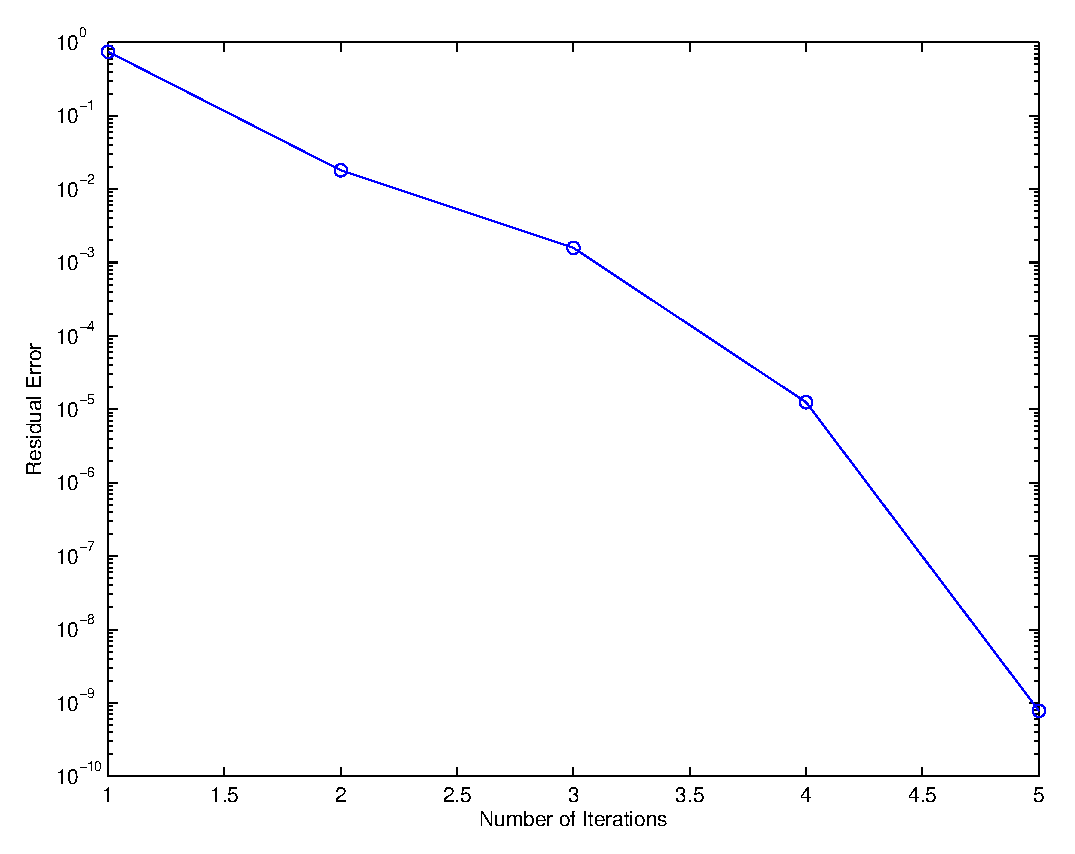
\includegraphics [scale = 0.5] {newtonfig.eps}}
%\caption{Convergence of Newton's Method}
%\end{minipage}\hfill
%\begin{minipage}{0.45\textwidth}
%\centerline{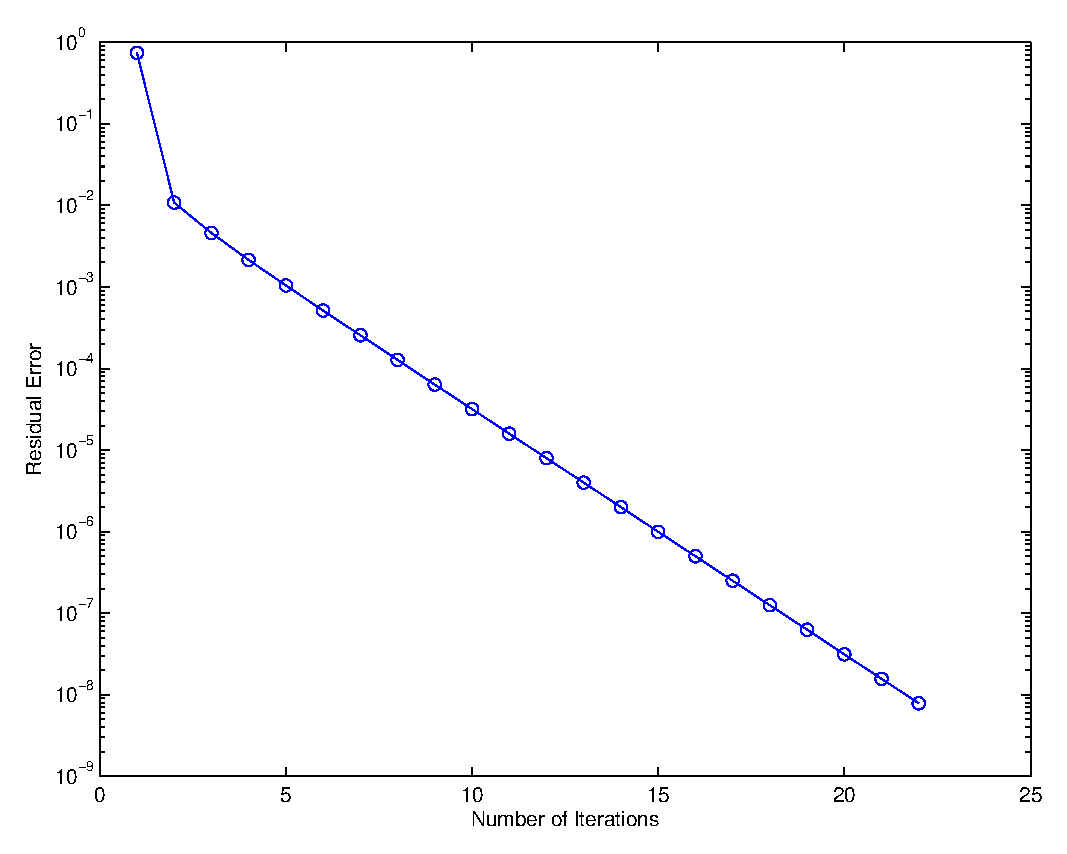
\includegraphics [scale = 0.5] {chordfig.eps}}
%\caption{Convergence of Chord Method}
%\end{minipage}\hfill
%\end{figure}

%\begin{figure}
%\begin{minipage}{0.45\textwidth}
%\centerline{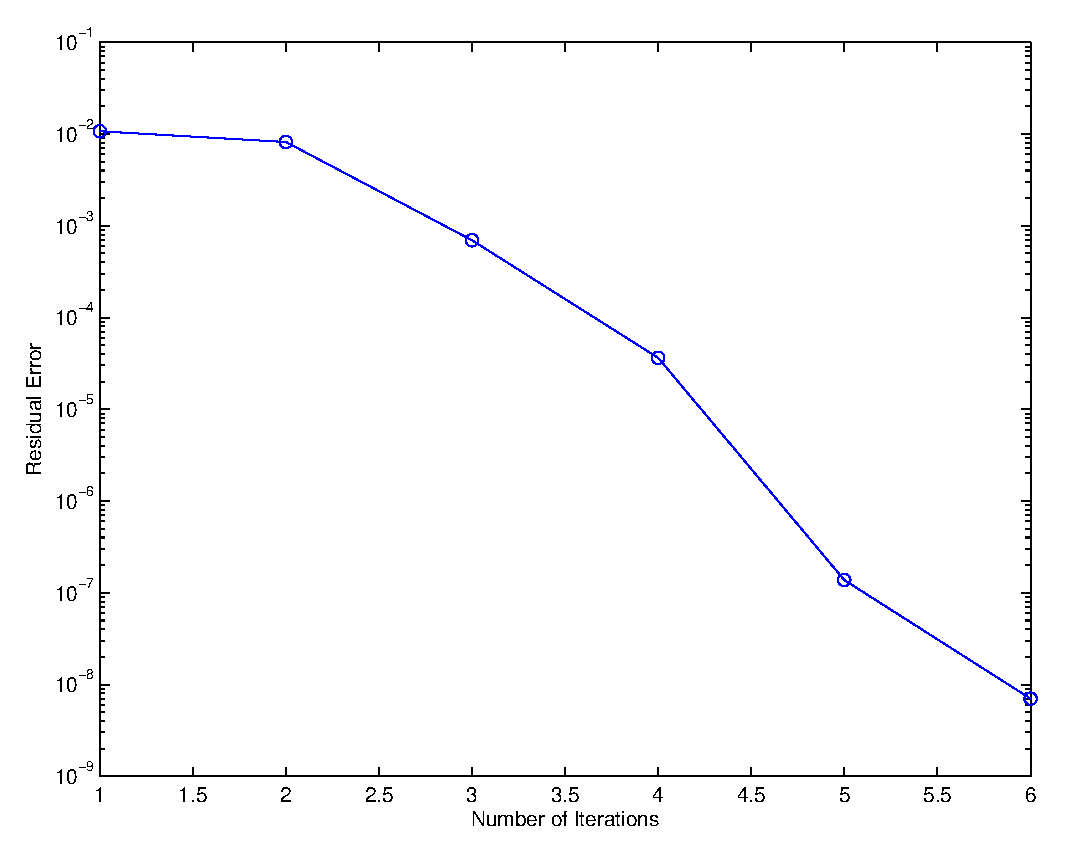
\includegraphics [scale = 0.5] {broydenfig.eps}}
%\caption{Convergence of Broyden's Method}
%\end{minipage}\hfill
%\begin{minipage}{0.45\textwidth}
%\centerline{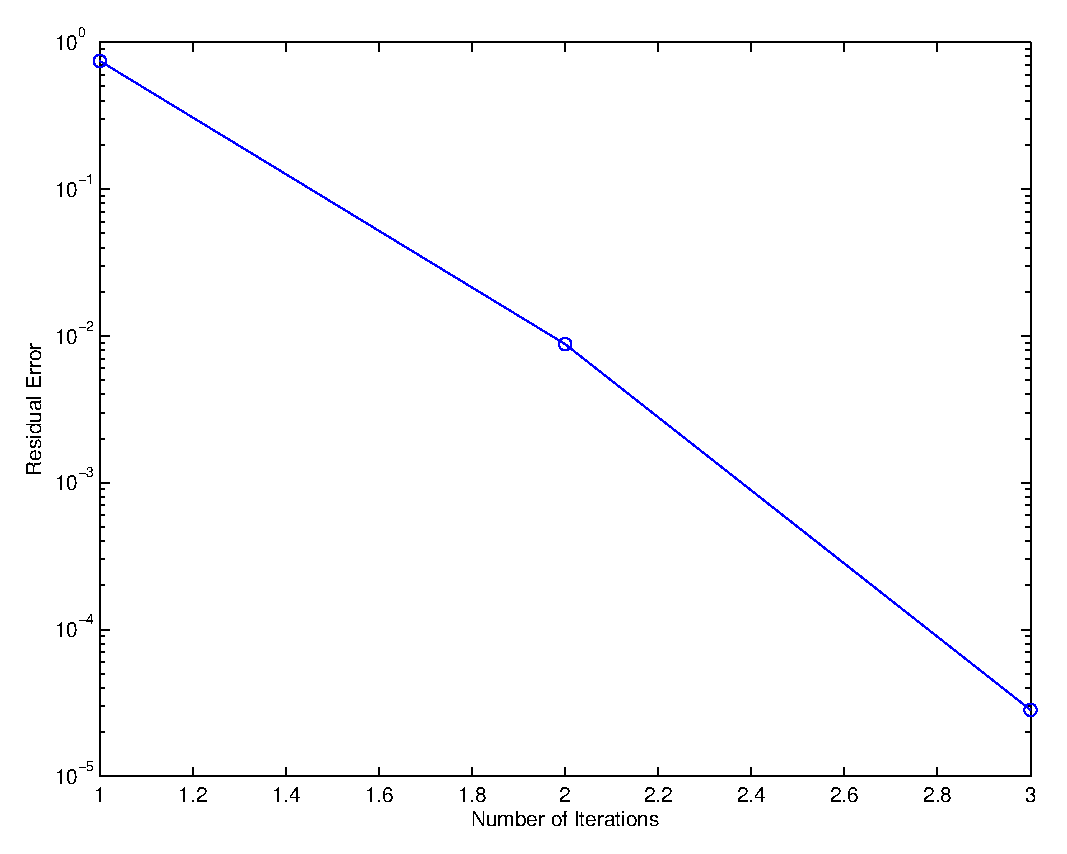
\includegraphics [scale = 0.5] {shamfig.eps}}
%\caption{Convergence of Shamanskii's Method}
%\end{minipage}\hfill
%\end{figure}

%\end{center}

\iffalse
\begin{center}

\begin{figure}[H]
\centerline{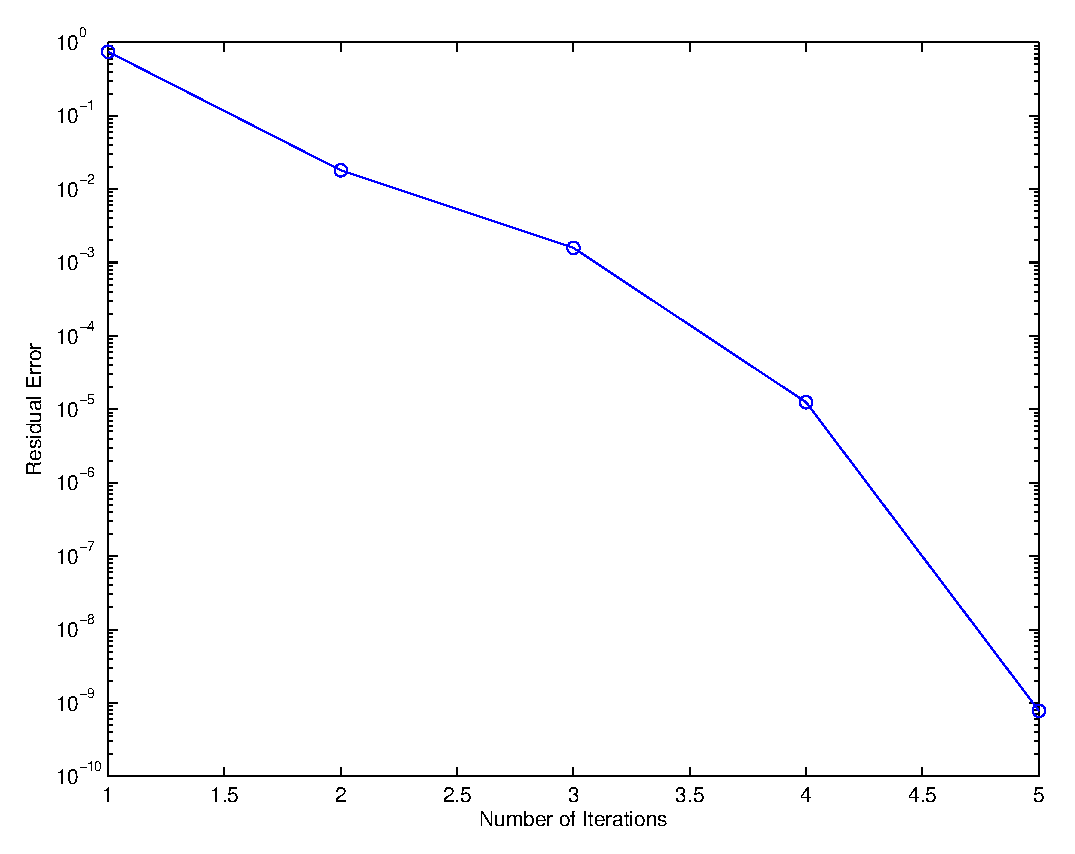
\includegraphics [scale = 0.5] {newtonfig.eps}}
\caption{Convergence of Newton's Method}
\end{figure}

\begin{figure}[H]
\centerline{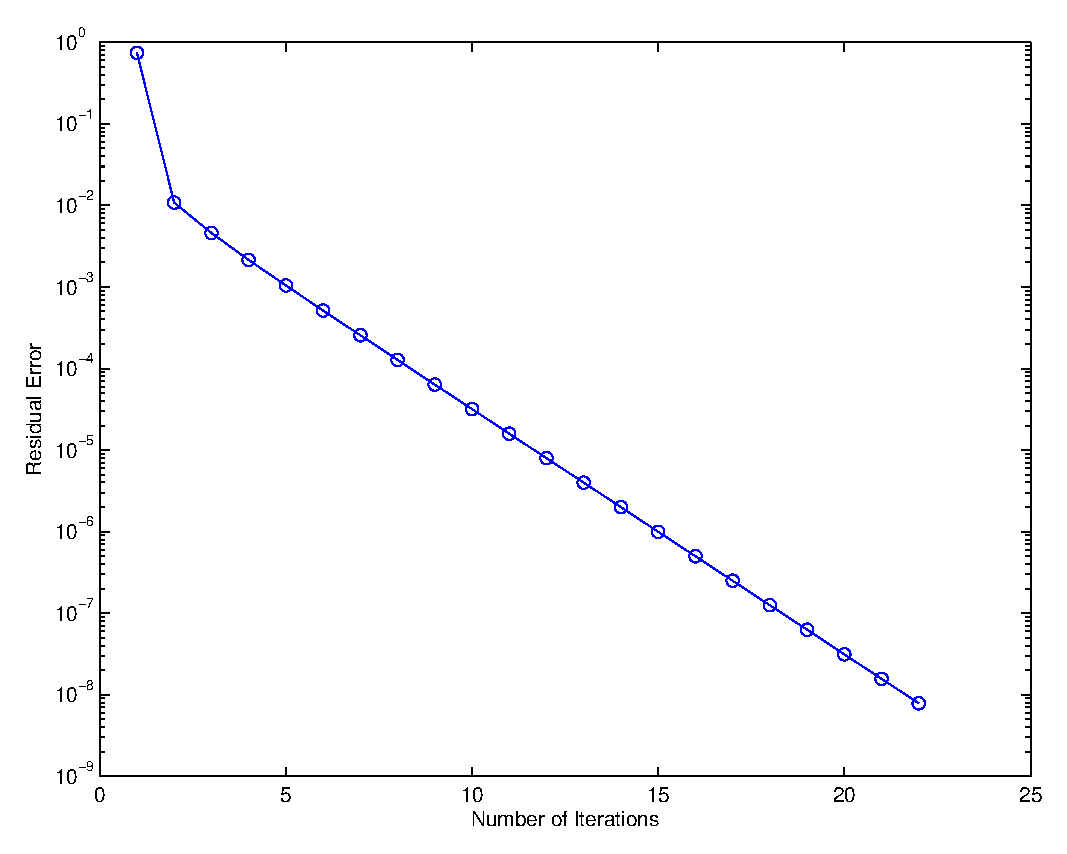
\includegraphics [scale = 0.5] {chordfig.eps}}
\caption{Convergence of Chord Method}
\end{figure}

\begin{figure}[H]
\centerline{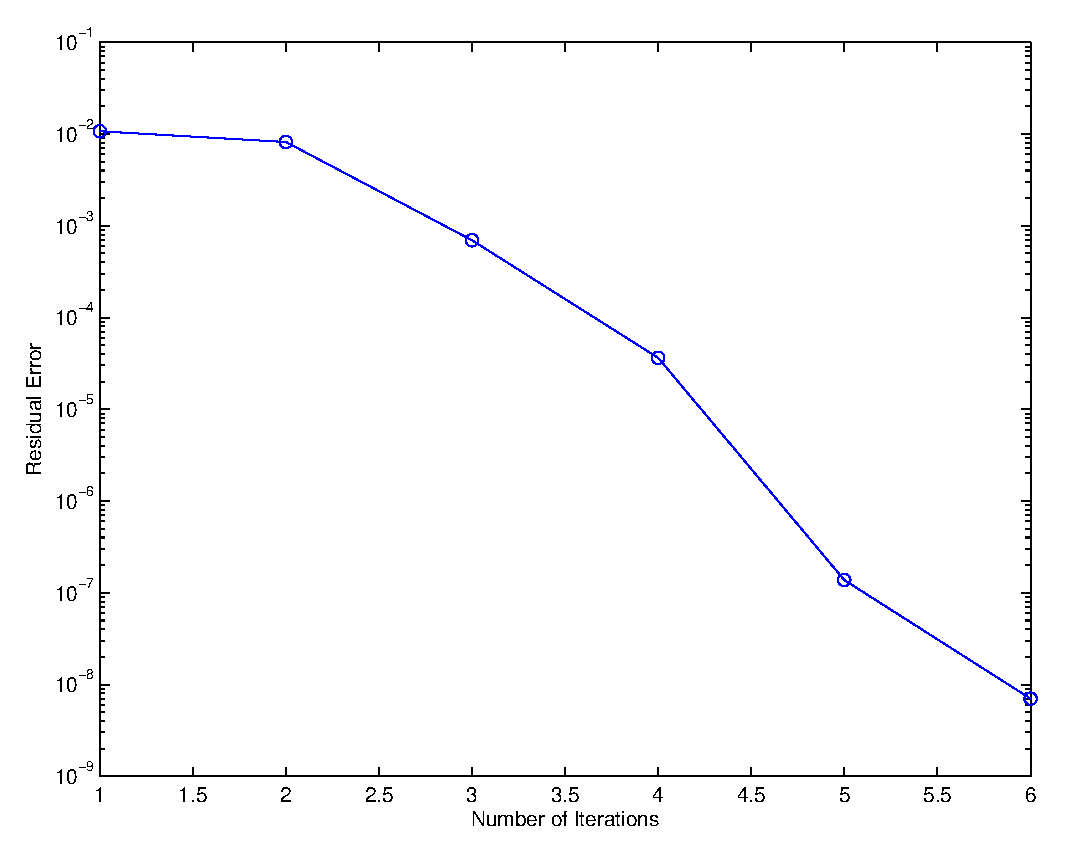
\includegraphics [scale = 0.5] {broydenfig.eps}}
\caption{Convergence of Broyden's Method}
\end{figure}

\begin{figure}[H]
\centerline{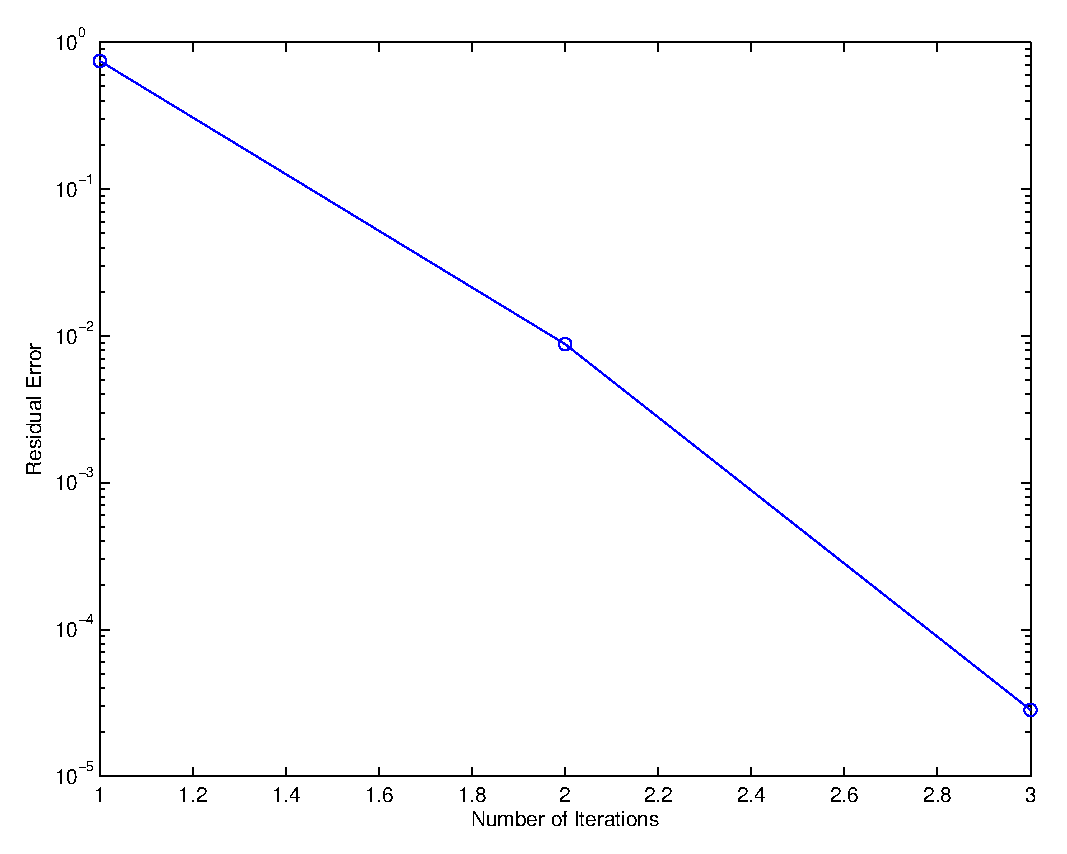
\includegraphics [scale = 0.5] {shamfig.eps}}
\caption{Convergence of Shamanskii's Method}
\end{figure}

\end{center}
\fi


\iffalse
\begin{figure}[H]
\begin{minipage}{0.5\textwidth}
\centerline{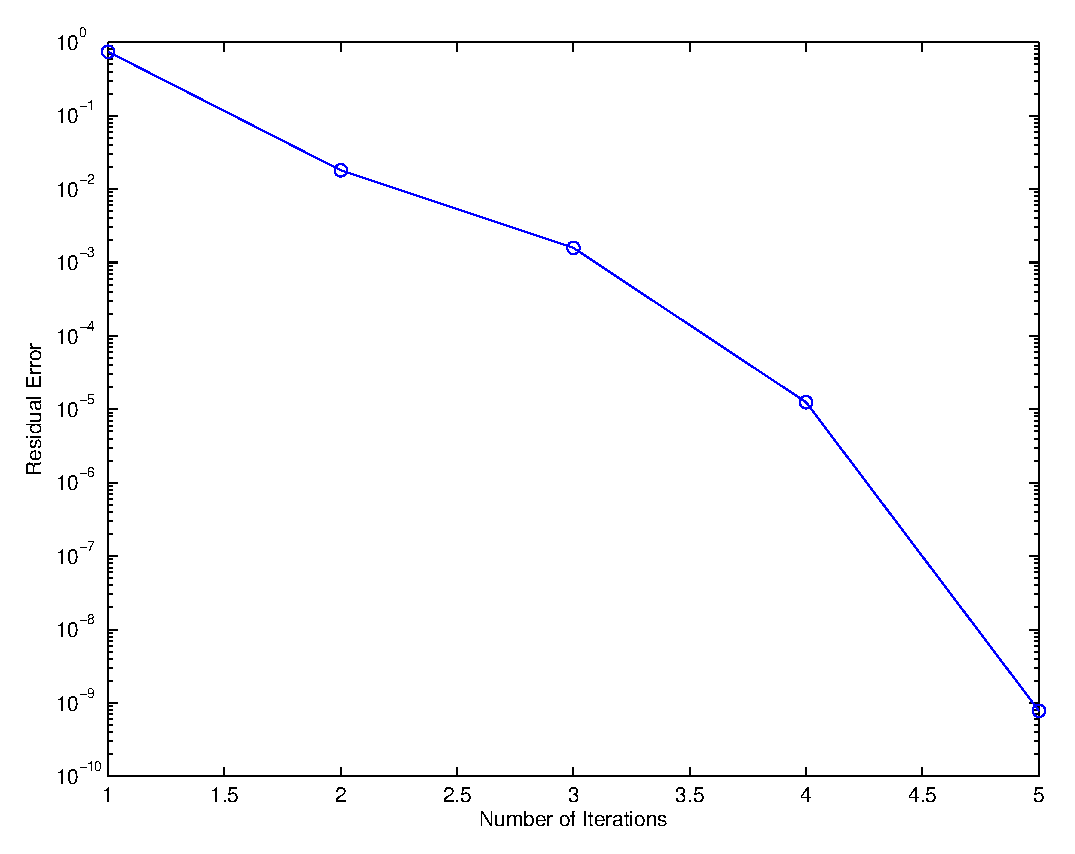
\includegraphics [scale = 0.4] {newtonfig.eps}}
\caption{Convergence of Newton's Method}
\end{minipage}
\begin{minipage}{0.5\textwidth}
\centerline{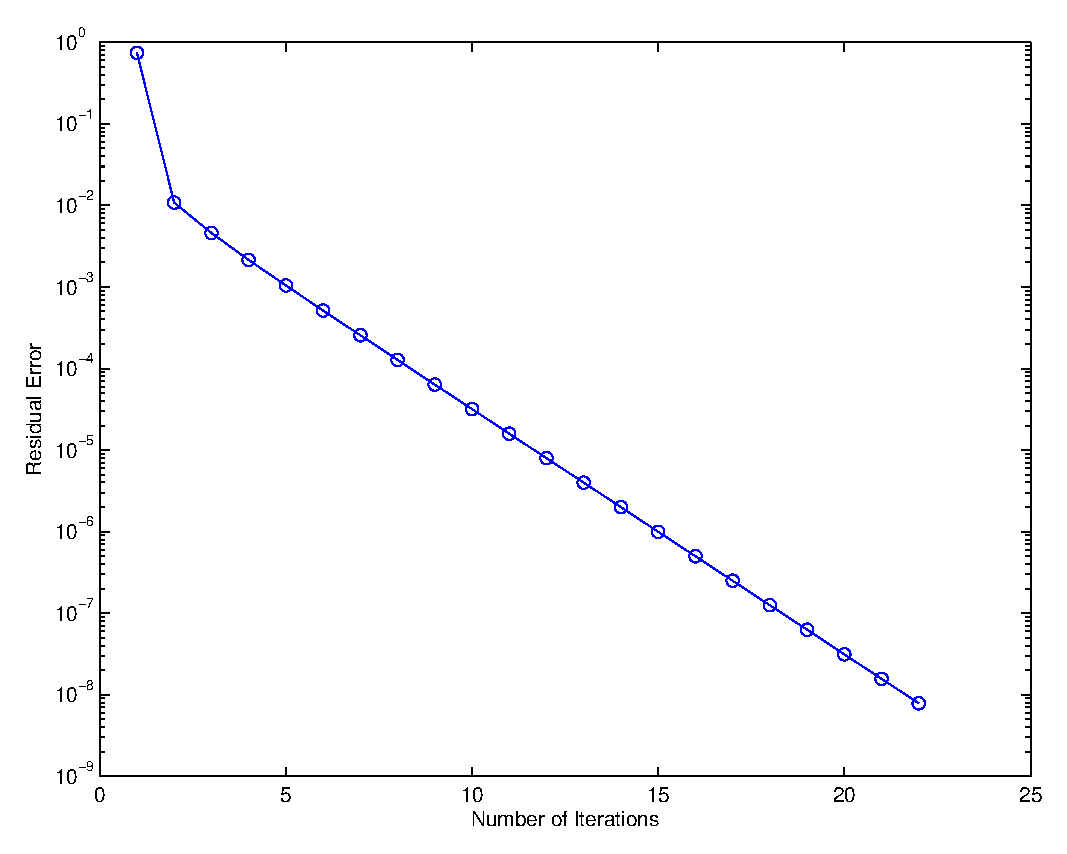
\includegraphics [scale = 0.4] {chordfig.eps}}
\caption{Convergence of Chord Method}
\end{minipage}
\end{figure}

\begin{figure}[H]
\begin{minipage}{0.5\textwidth}
\centerline{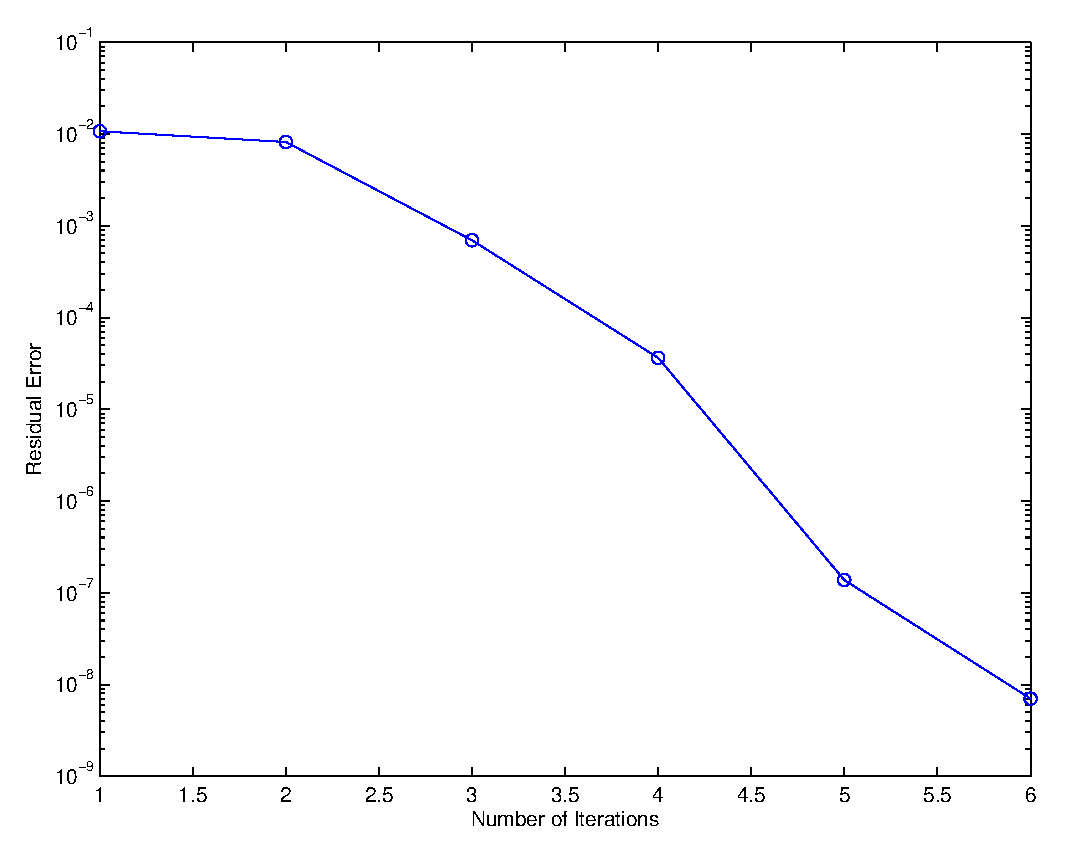
\includegraphics [scale = 0.4] {broydenfig.eps}}
\caption{Convergence of Broyden's Method}
\end{minipage}
\begin{minipage}{0.5\textwidth}
\centerline{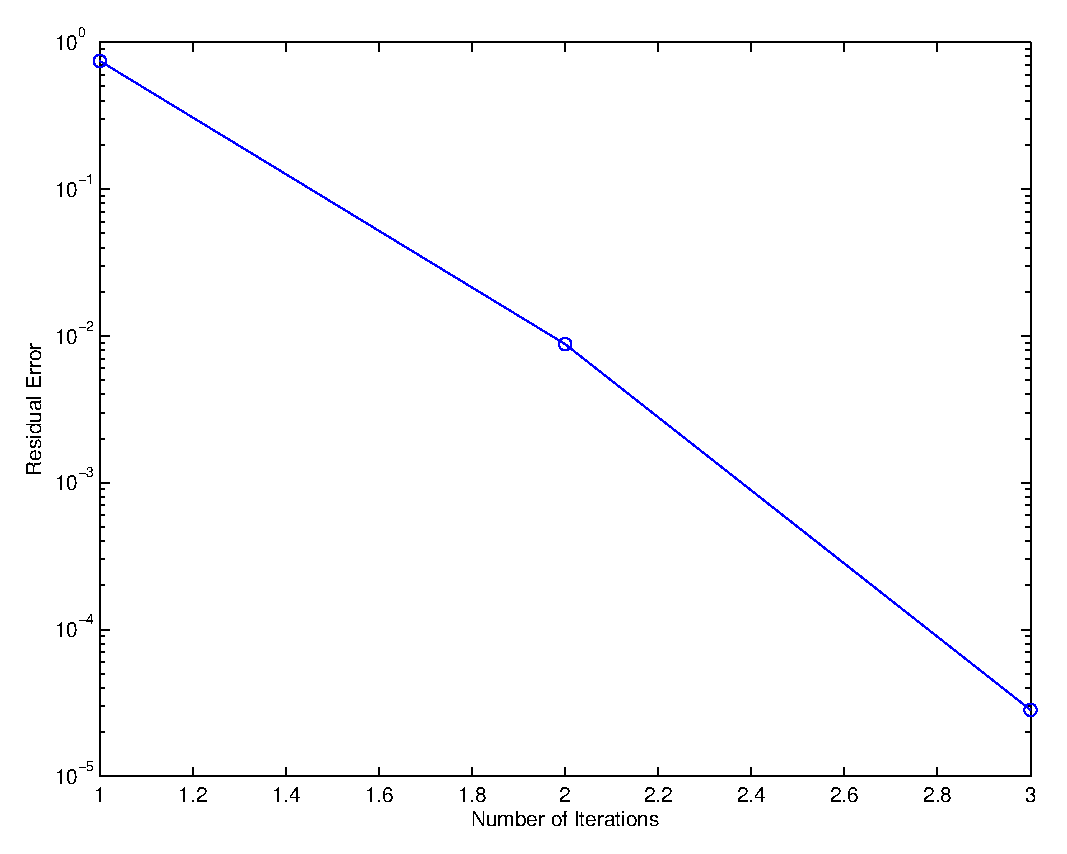
\includegraphics [scale = 0.4] {shamfig.eps}}
\caption{Convergence of Shamanskii's Method}
\end{minipage}
\end{figure}
\fi

% FINAL FIGURES

\begin{figure}[H]
\begin{subfigure}{.5\textwidth}
\centering
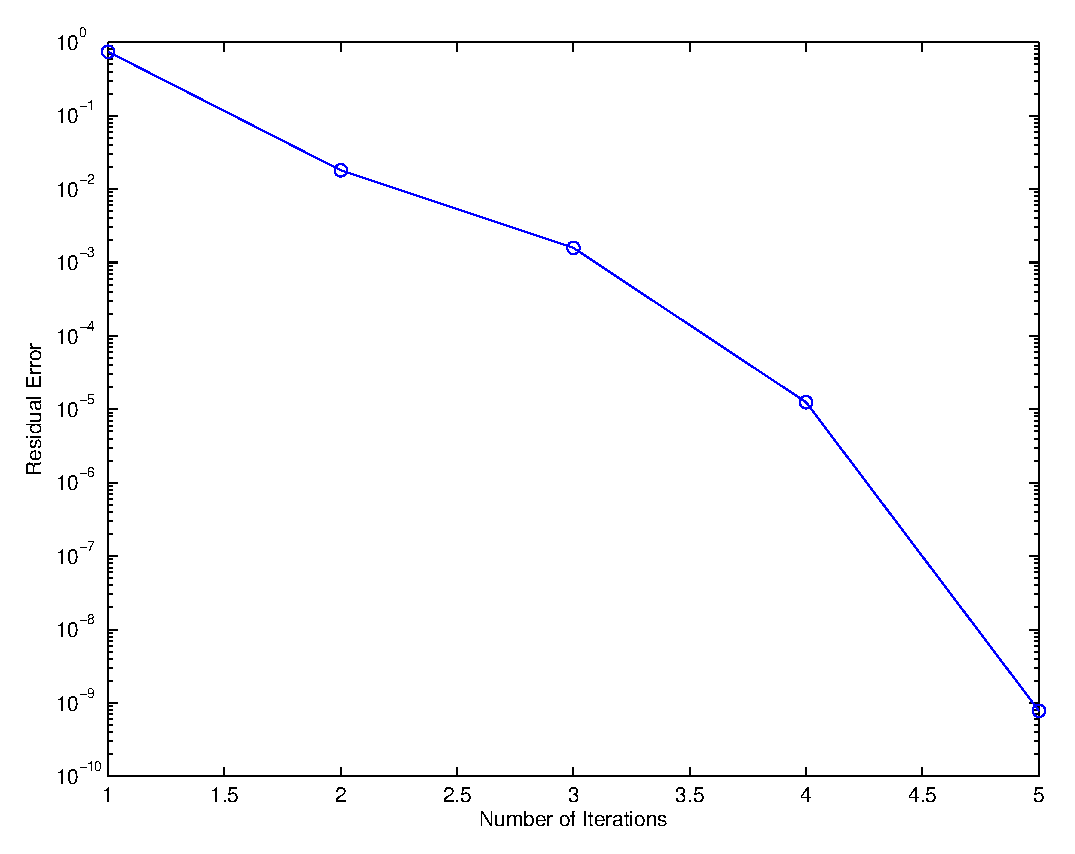
\includegraphics [width = 1\linewidth] {newtonfig.eps}
\caption{Convergence of Newton's Method}
\end{subfigure}
\begin{subfigure}{.5\textwidth}
\centering
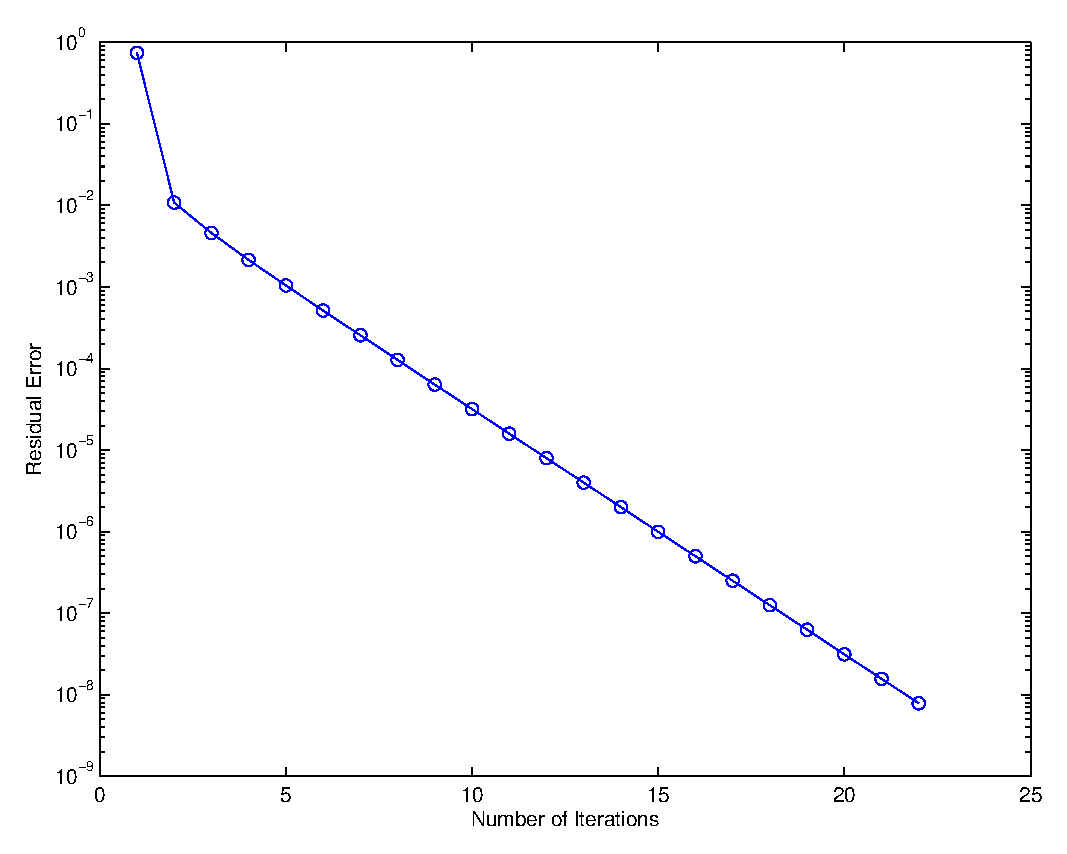
\includegraphics [width = 1\linewidth] {chordfig.eps}
\caption{Convergence of Chord Method}
\end{subfigure}
\end{figure}

\begin{figure}[H]
\begin{subfigure}{.5\textwidth}
\centering
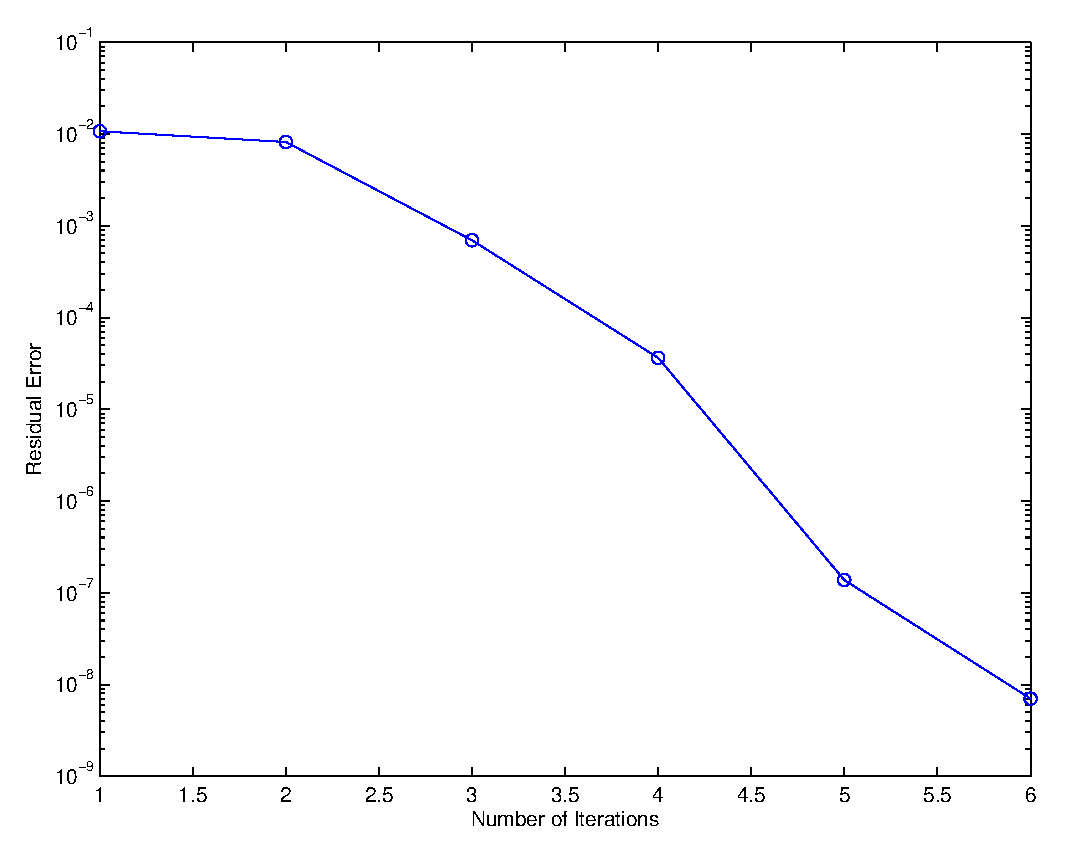
\includegraphics [width = 1\linewidth] {broydenfig.eps}
\caption{Convergence of Broyden's Method}
\end{subfigure}
\begin{subfigure}{.5\textwidth}
\centering
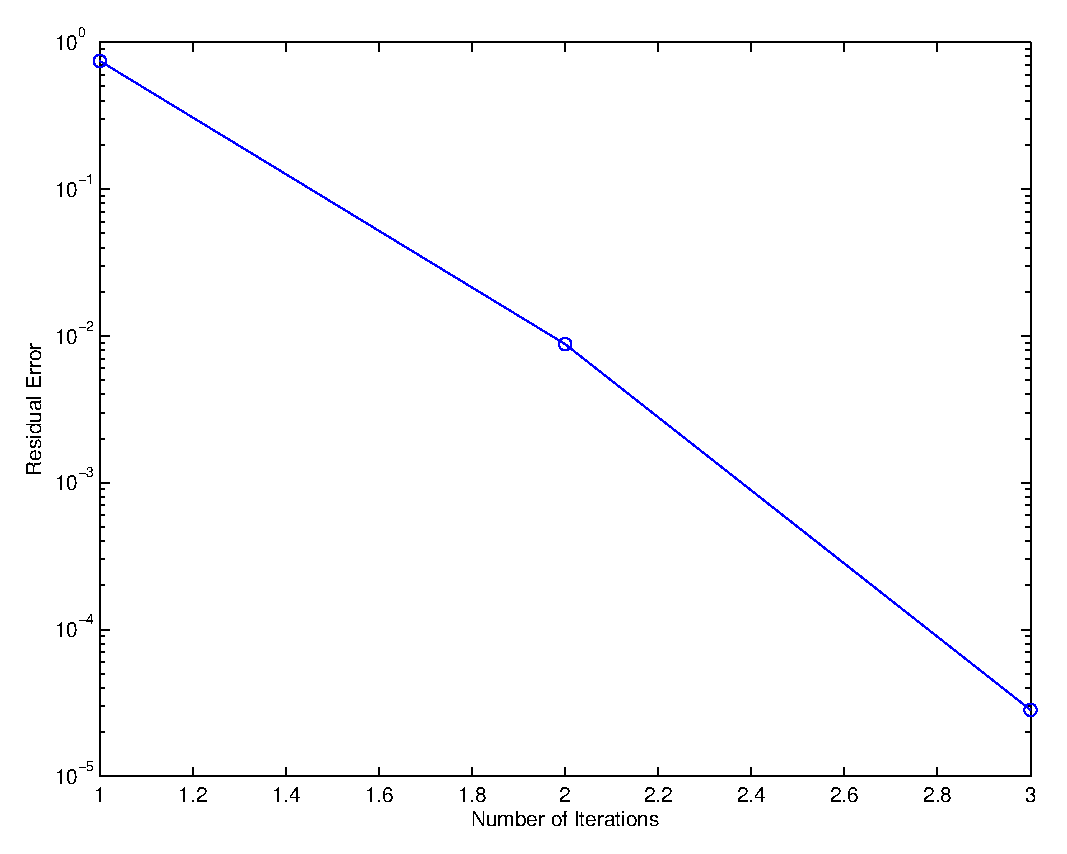
\includegraphics [width = 1\linewidth] {shamfig.eps}
\caption{Convergence of Shamanskii's Method}
\end{subfigure}
\end{figure}


\section{Conclusion}
In conclusion, Newton's method and it's variations are all very fast algorithms for finding the roots of nonlinear systems of equations.  Each have their own strengths and weaknesses depending on what the desired result is.  For example, the Chord method sacrifices accuracy in order to reduce the compuational complexity of recalculating the Jacobian matrix on every iteration, whereas Broyden's method only evaluates it once but makes new approximations on every iteration in order to quickly and accurately complete the algorithm.  It's not possible to say that one of these methods is better than another, as they can all be appropriate depending on resources and desired outcome.  


\clearpage

\bibliography{mybib} { }
\bibliographystyle{plain}















% --------END DOCUMENT-----------%

\end{document}